% -%-%-%-%-%-%-%-%-%-%-%-%-%-%-%-%-%-%-%-%-%-%-%-%-%
% MDI224 % 
% Data:08/02/2012                                 %
% Paris,France                                    % 
% Groupe:                                         %
% - Tiago Chedraoui Silva                   % 
% - Anthony CLERBOUT
% -%-%-%-%-%-%-%-%-%-%-%-%-%-%-%-%-%-%-%-%-%-%-%-%-%

\documentclass[a4paper,11pt]{article}

\usepackage[francais,listings,algo]{tcs}

% Cover %
\def \ttprofname{Roland BADEAU} % teachers name
\def \ttabrv{MDI224} % abbreviation of names class
\def \ttabrvxt{} % period
\def \mytitle{Optimisation de portefeuille} % Big title
\def \mysubtitle{Travaux Pratique 3 - Deuxième semestre de 2012} % subtitle
\def \ttauthi{Anthony CLERBOUT} % author's name
\def \ttxti{Casier: 234} % Extra text right side of name
\def \ttauthii{Tiago CHEDRAUOI SILVA} % author's name
\def \ttxtii{Casier: 214 } % Extra text right side of name
\def \ttdate{Février 6, 2011} % date

\begin{document}
\titleTMB 
\newpage
\tableofcontents
\listoffigures
\newpage

\section{Frontière de marché}

\subsection{Estimation des caractéristiques du marché}

La  fonction ``mean''  a été  utilisé pour  qu'on puisse  trouver le  vecteur de
rendement moyen. Pour la matrice de covariance on a fait:

\begin{equation*}
Q = \mathbb{E}[(R-m)*(R-m)^{t}]
\end{equation*}

Ces  fonctions  peuvent être  vue  dans  le début  du  code  Ventes à  découvert
autorisées dans la prochaine section.

\subsection{Ventes à découvert autorisées}

Le problème d'optimisation est de  minimiser le risque pour un certain rendement
souhaité.

\begin{eqnarray*}
min J(x)&=& \frac{x^tQx}{2}\\
u^tx&=&1\\
x^tm&\geq&Re
\end{eqnarray*}

Le lagrangien du problème est:

\begin{eqnarray*}
L(x,\lambda,\mu)&=& \frac{x^tQx}{2}+ \lambda (u^tx-1)+ \mu(Re-x^tm)\\
\delta_xL&=&Qx + \lambda u - \mu m = 0\\
\end{eqnarray*}

Donc:


\begin{eqnarray*}
x &=& \mu Q^{-1}m - \lambda Q^{-1} u
\end{eqnarray*}

En utilisant ce x dans le contraintes, on ira avoir le système suivant:

\begin{eqnarray*}
\begin{pmatrix}
  \mu &  \\
  \lambda
 \end{pmatrix} 
={1 \over B^2-DA}\begin{pmatrix}
  B & -A\\
  -D & B
 \end{pmatrix} 
\begin{pmatrix}
  1 &  \\
  Re
 \end{pmatrix} 
\end{eqnarray*}
 
Avec le $\mu$ et $\lambda$, on peut calculer le $x^*$ et $\sigma ^*$, mais il existe deux cas,
un quand $Re<B/A$ et d'autre quand $Re\geq B/A$.

\begin{eqnarray*}
Re&\geq& B/A\\
x^* &=& \mu Q^{-1}m - \lambda Q^{-1} u\\
\sigma ^* &=& x^*Qx=f(Re)
\end{eqnarray*}


\begin{eqnarray*}
Re&<& B/A\\
x^* &=& \frac{Q^{-1}u}{u^tQ^{-1}u}\\
\sigma ^* &=& \sqrt{\frac{1}{u^tQ^{-1}u}}
\end{eqnarray*}

Le code pour ces calculs est au dessous.
\begin{multicols}{2}
  \lstinputlisting[title=\textbf{Ventes à découvert autorisées}]{../code/redement.m}
\end{multicols}

\newpage
La figure  au dessous affiche la  frontière du marché pour  un nombre différents
d'actifs. On peut voir que pour un rendement fixe, plus d'actifs implique un 
risque plus petite.


\begin{figure}[h!]
  \begin{centering}
    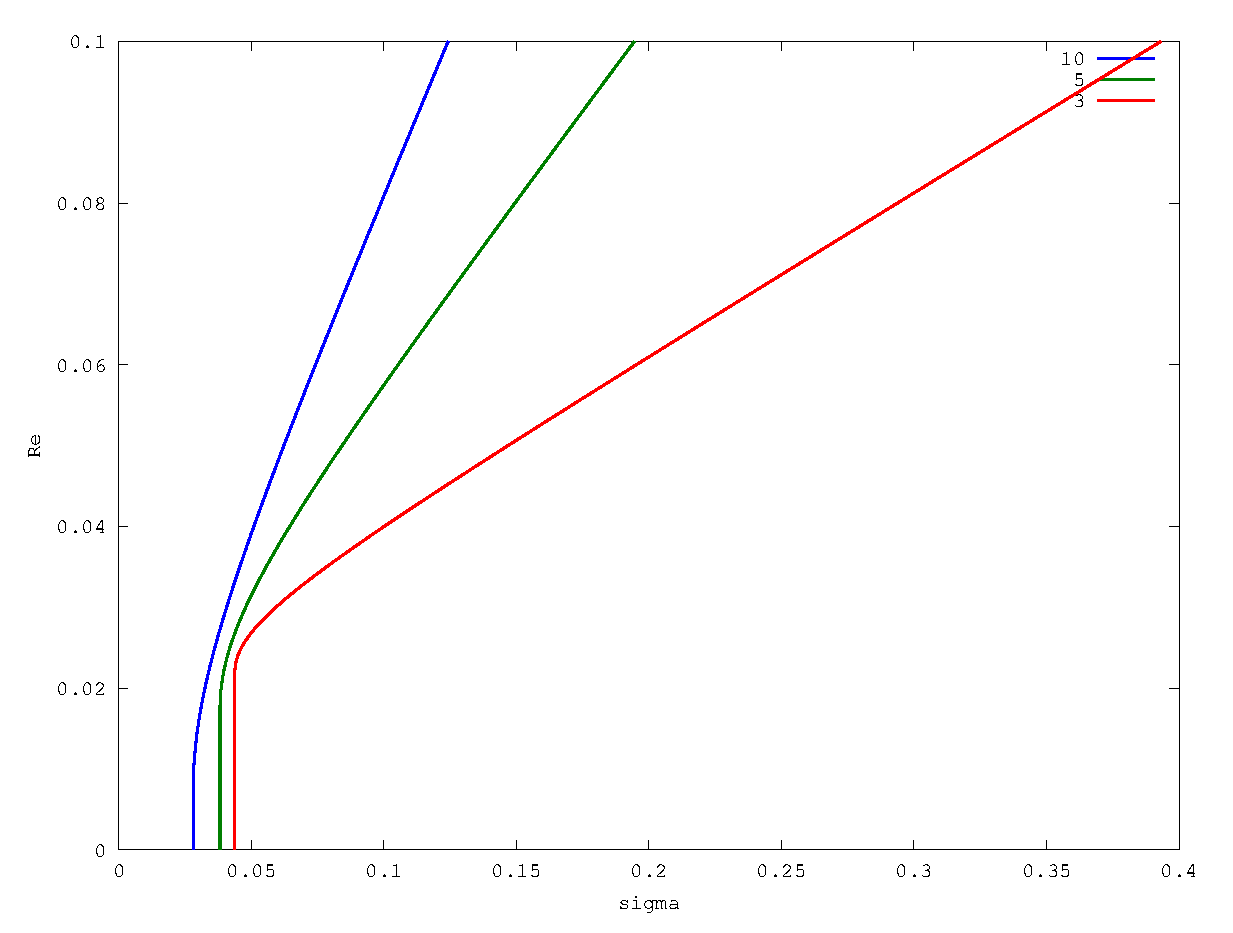
\includegraphics[scale=0.4]{redment10.eps}
    \label{rspro2}
    \par\end{centering}
  \caption{Frontière du marché pour un nombre différent d'actifs}
  \label{fig:jacobi-conv}
\end{figure}

En suite, on a pris deux actifs et on a varier leur corrélation entre -0.9 et 0.9. Voir le code au dessous.

\begin{multicols}{2}
  \lstinputlisting[title=\textbf{Ventes à découvert autorisées}]{../code/rendCov.m}
\end{multicols}


La  figure au dessous affiche le  rendement en fonction du  risque pour un
portefeuille à 2 actifs pour différentes valeurs de la corrélation.

\begin{figure}[h!]
  \begin{centering}
    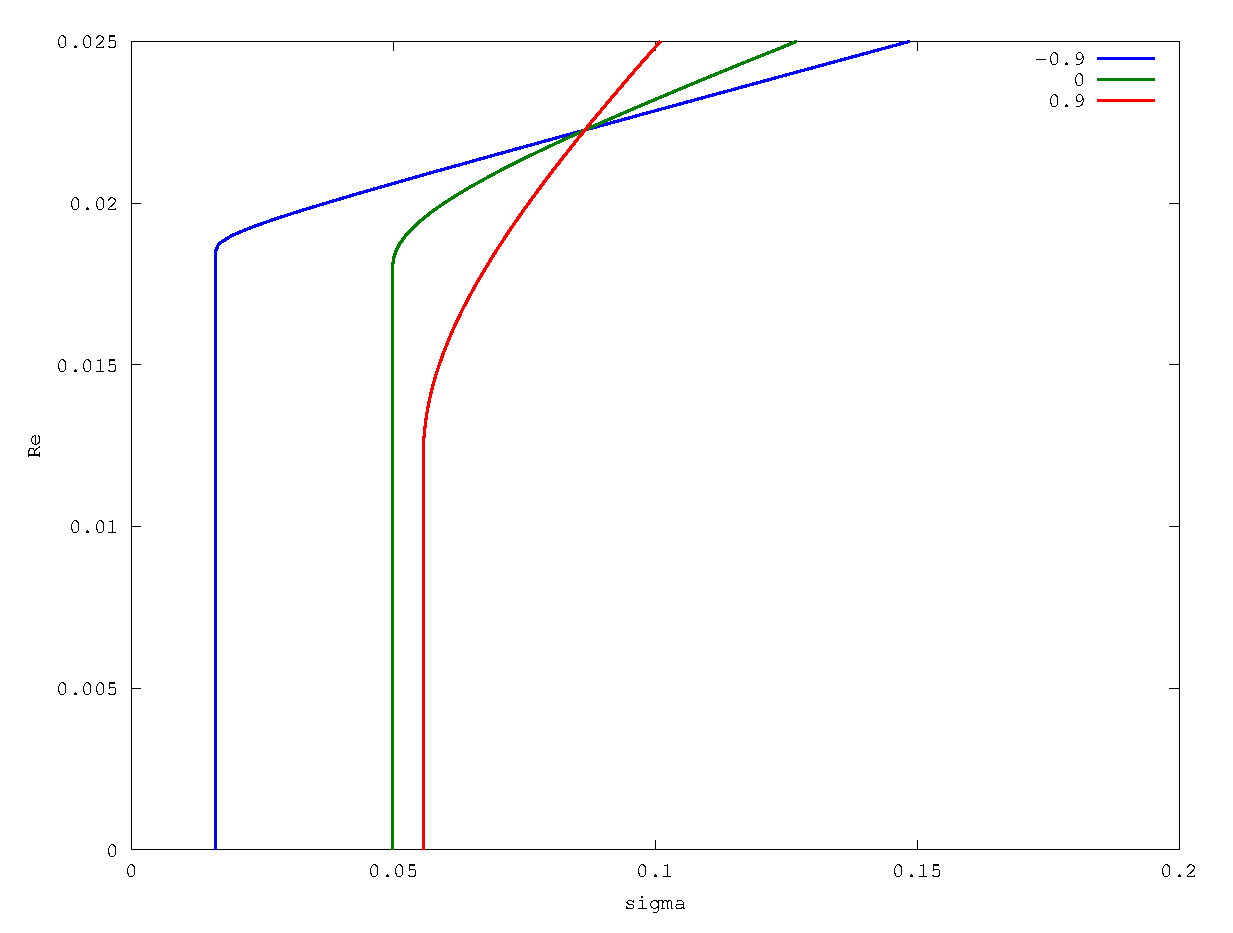
\includegraphics[scale=0.4]{rho.eps}
    \label{rspro2}
    \par\end{centering}
  \caption{Rendement en fonction du risque pour un portefeuille à 2 actifs pour différentes valeurs de la corrélation.}
  \label{fig:jacobi-conv}
\end{figure}

\newpage

\subsection{Ventes à découvert non autorisées}
Pour que le  problème ait une solution, le rendement avec  la moyenne plus grand
doit être plus  grand que $R_e$, cela  veut dire, si on investisse  tout dans ce
actif on peut avoir un rendement plus haut que $R_e$, par contre en ajoutant des
actifs avec un rendement plus petite $x^tm$ ira diminuer.

Ainsi, pour  qu'il existe au  moins une solution,  le $max_i m_i$ doit  être plus
grande que $R_e$ et $x_0$ sera un  vecteur que a un investissement de 100\% dans
$max_i m_i$. On peut facilement que ce x  satisfait les contraintes.

Comme a ce moment les ventes à découvert sont non autorisées, cela veut dire que
notre problème sera:
\begin{eqnarray*}
min J(x)&=& \frac{x^tQx}{2}\\
u^tx&=&1\\
x^tm&\geq&Re\\
x&\geq&0
\end{eqnarray*}

Ainsi, en utilisant la fonction QPactivate.m pour tracer la frontière du marcher, le code suivante a été crée.:

\begin{multicols}{2}
  \lstinputlisting[title=\textbf{Ventes à découvert non autorisées}]{../code/noauto.m}
\end{multicols}
Comme résultat, on a la figure suivante:

\begin{figure}[h!]
  \begin{centering}
    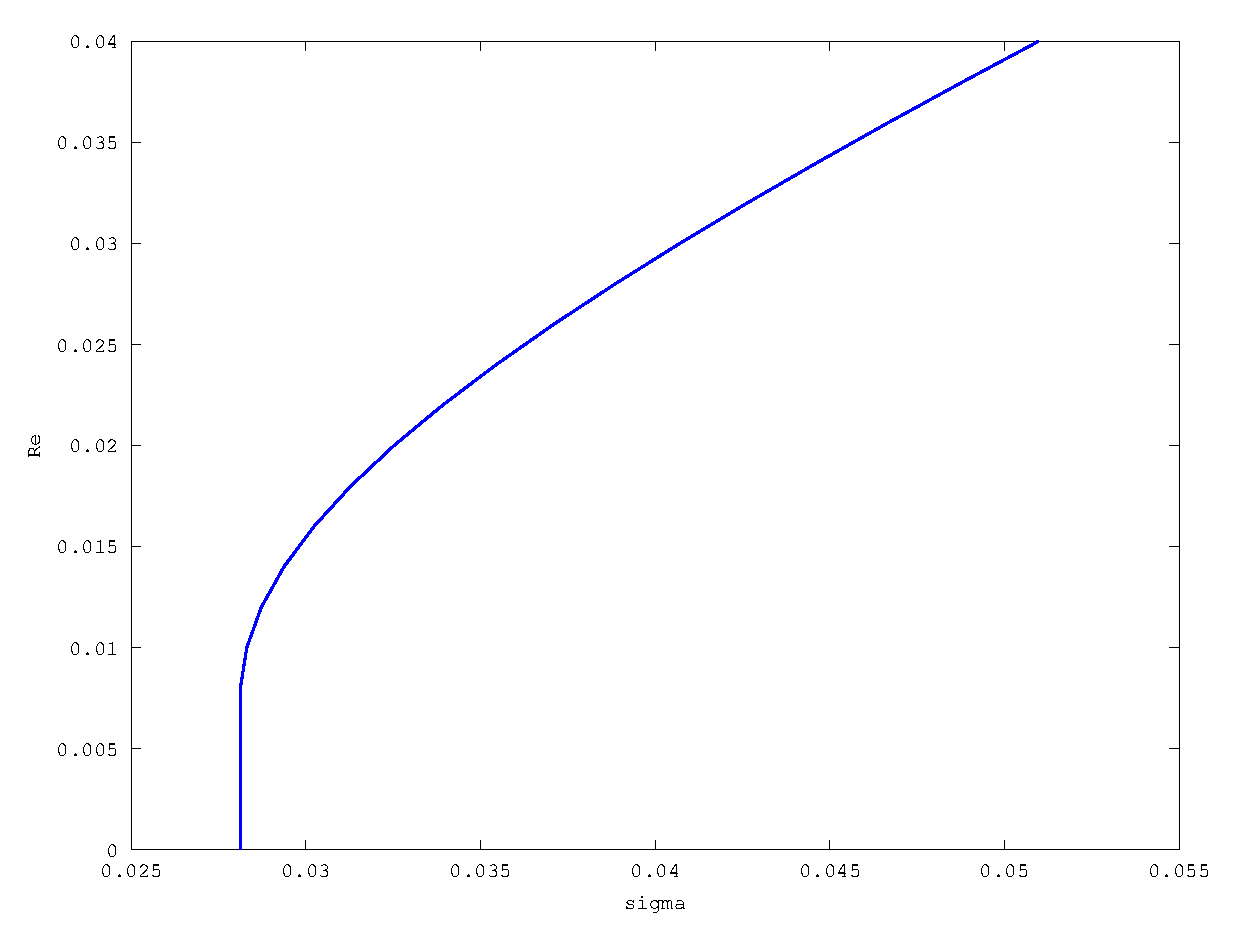
\includegraphics[scale=0.4]{parte14.eps}
    \par\end{centering}
  \caption{Rendement  en  fonction du  risque  pour  un  portefeuille: ventes  a
    découverte autorisées.}
  \label{fig:jacobi-conv}
\end{figure}


% ratio de sharp 11.449?
\end{document}

